\subsection{Replication}


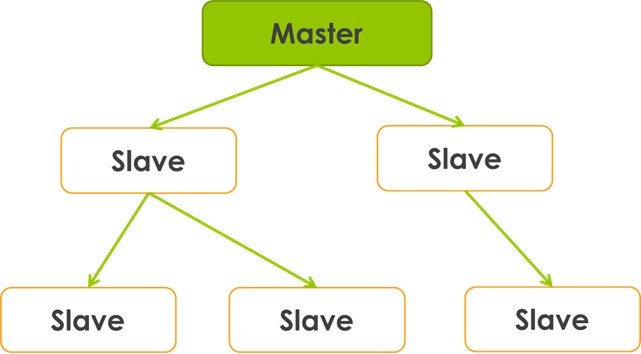
\includegraphics{images/Redis_Master_N_Slaves_Replikation.jpg}
 \cite{RedisReplicationPicture}

Redis uses a Master-N-Slave-replication. Here are some important facts:

\begin{itemize}
  \item It is possible to have as many slaves as you want in row or in series.
  \item The slaves synchronize with the master.
  \item Redis uses asynchronous replication.
  \item Replication can be used for scalability (slaves can be used for very slow read operations) or just for data redundancy.
  \item If the master falls out, one slave can become new master.

\end{itemize}


 \cite{RedisReplication}


